\documentclass[11pt]{a0poster}
\usepackage[top=1.6cm, bottom=1.6cm, left=1.6cm, right=1.6cm]{geometry} 
%\usepackage{geometry}                % See geometry.pdf to learn the layout options. There are lots.
\geometry{a0paper}                   % ... or a4paper or a5paper or ... 
\geometry{portrait}                % Activate for for rotated page geometry
%\usepackage[parfill]{parskip}    % Activate to begin paragraphs with an empty line rather than an indent
\usepackage{authblk}
\usepackage[pdftex]{graphicx}
\usepackage{amssymb}
\usepackage{float}
\usepackage{ifpdf}
\usepackage{multicol}
\usepackage{url}
\ifpdf
   \usepackage{epstopdf}
   \usepackage{pdfsync}
\fi
\usepackage{fix-cm}

\usepackage{wrapfig}
\DeclareGraphicsRule{.tif}{png}{.png}{`convert #1 `basename #1 .tif`.png}
\renewcommand{\familydefault}{\sfdefault}

\title{ \fontsize{56}{72}\selectfont {\bf Integration of CBF, NeXus and HDF5}\vspace{-10mm} }
\author[a]{ \fontsize{20}{24}\selectfont Herbert J. Bernstein}
\author[b]{ \fontsize{20}{24}\selectfont Jonathan M. Sloan}
\author[b]{ \fontsize{20}{24}\selectfont Graeme Winter}
\author[b]{ \fontsize{20}{24}\selectfont Tobias S. Richter}
\author[c]{ \fontsize{20}{24}\selectfont NeXus International Advisory Committee}
\author[d]{ \fontsize{20}{24}\selectfont Committee on the Maintenance of the CIF Standard}

\affil[a]{ \fontsize{16}{20}\selectfont Department of Mathematics and Computer Science, Dowling College, Oakdale, NY 11769 (USA). }
\affil[b]{ \fontsize{16}{20}\selectfont Diamond Light Source, Harwell Science and
Innovation Campus, OX11 0DE (UK)}
\affil[c]{ \fontsize{16}{20}\selectfont {http://wiki.nexusformat.org/NIAC}}
\affil[d]{ \fontsize{16}{20}\selectfont {http://www.iucr.org/resources/cif/comcifs}}

\date{}                                           
% Activate to display a given date or no date

\begin{document}
%\maketitle
\begin{titlepage}
\end{titlepage}
\begin{minipage}[]{\linewidth}
\begin{center}
~~{\fontsize{43}{53}\selectfont\bf Coping {\fontsize{43}{53}\selectfont\bf with} BIG DATA Image Formats: {\fontsize{43}{53}\selectfont\bf Integration of} CBF, NeXus {\fontsize{43}{53}\selectfont\bf and} HDF5, A Progress Report}
~~\\
\vspace{8mm}
{\fontsize{30}{36}\selectfont Herbert J. Bernstein,$^{\dagger}$}
{\fontsize{30}{36}\selectfont Jonathan M. Sloan,$^{\star}$}
{\fontsize{30}{36}\selectfont Graeme Winter,$^{\star}$}
{\fontsize{30}{36}\selectfont Tobias S. Richter,$^{\star}$}
{\fontsize{30}{36}\selectfont NeXus International Advisory Committee,$^{\ddag}$}
{\fontsize{30}{36}\selectfont Committee on the Maintenance of the CIF Standard$^{\Psi}$}
\end{center}
\end{minipage}\\
\begin{minipage}[]{0.02\linewidth}~\end{minipage}\hfill%
\begin{minipage}[]{.29\linewidth}
\begin{figure}[H]
\begin{center}
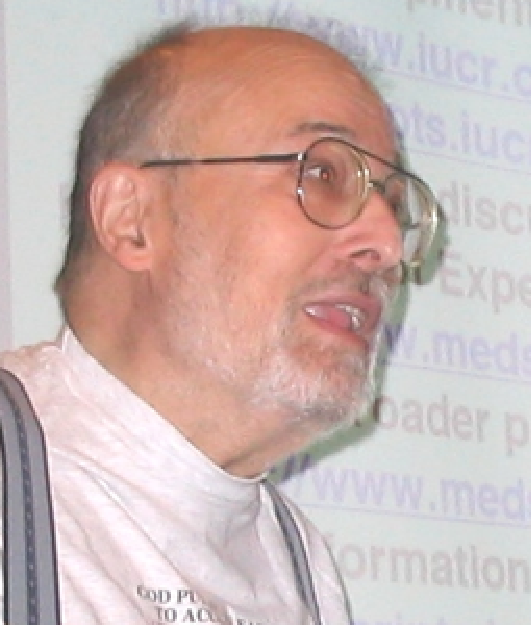
\includegraphics[width=50mm]{Bernstein_Herbert}
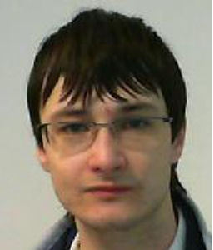
\includegraphics[width=50mm]{Sloan_Jonathan}
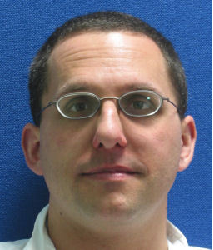
\includegraphics[width=50mm]{Winter_Graeme}
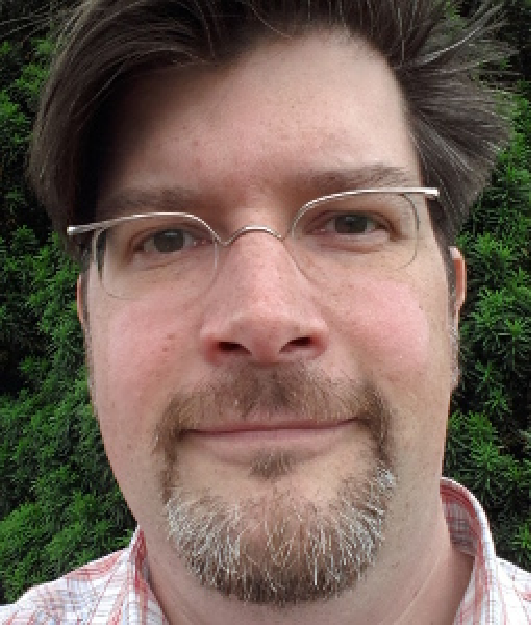
\includegraphics[width=50mm]{Richter_Tobias}
\end{center}
\end{figure}

\end{minipage}\hfill%
\begin{minipage}[]{.4\linewidth}
\begin{center}
\vspace{8mm}

{\fontsize{24}{28}\selectfont $^{\dagger}$Department of Mathematics and Computer Science, Dowling College, Oakdale, NY 11769 (USA)}

{\fontsize{24}{28}\selectfont $^{\star}$Diamond Light Source, Harwell Science and
Innovation Campus, OX11 0DE (UK)}

{\fontsize{24}{28}\selectfont $^{\ddag}${http://wiki.nexusformat.org/NIAC}}

{\fontsize{24}{28}\selectfont $^{\Psi}${http://www.iucr.org/resources/cif/comcifs}}
\vspace{4mm}
\end{center}
\end{minipage}\hfill%
\begin{minipage}[]{.10\linewidth}
\begin{figure}[H]
\begin{center}
\vspace{-10mm}
\includegraphics[width=60mm]{Pilatus3a}
{~~\\
\vspace{-8mm}
Dectris Pilatus3 6M}
\end{center}
\end{figure}
\end{minipage}\hfill%
\begin{minipage}[]{.10\linewidth}
\begin{figure}[H]
\begin{center}
\hspace{-10mm}\includegraphics[width=60mm]{cspad}
{~\\
\vspace{-2mm}
Cornell-SLAC pixel array detector (CSpad) }
\end{center}
\end{figure}
\end{minipage}
\\
\fontsize{18}{22}\selectfont
\begin{minipage}[]{0.01\linewidth}~\end{minipage}\hfill\begin{minipage}[]{0.29\linewidth}
\fontsize{18}{22}\selectfont
\begin{figure}[H]
\vspace{-15mm}
\begin{center}
      {
\fontsize{16}{20}\selectfont ~~\\
Abstract 1.2.4\_1995
24 -- 28 May 2014 at American Cryst. Assoc. meeting, Albuquerque, NM USA.\\
Work supported in part by NIGMS, DOE, NSF, PaNdata ODI (EU 7th Framework Programme)}
\end{center}
\end{figure}

\vspace{1mm}
%\section*{Introduction}

\fontsize{18}{22}\selectfont%

\begin{wrapfigure}{r}{0.40\textwidth}
\begin{center}
\vspace{-20 mm}
\includegraphics[width=4.5in]{Eigera}
\vspace{-20 mm}
\caption{\fontsize{16}{20}\selectfont %
Dectris Eiger 1M, an example of the new generation
of very high data rate detectors that raise BIG DATA
issues.
}
\label{fig:eiger}
\end{center}
\end{wrapfigure}
The BIG DATA demands of the new generation of X-ray pixel array detectors
necessitate the use of new storage technologies as we meet the limitations of
existing file systems. Fast Dectris Pilatus detectors and FEL detectors such as
the Cornell-SLAC pixel array detector (CSPAD) are already straining
file systems, and the new generation of even faster detectors, such as the Dectris Eiger
shown in Fig. 1,
will bring this issue to a head. In addition, the modular
nature of these detectors provides the opportunity
to construct more complex detector arrays (e.g. the
Dectris Pilatus detector at I23 at DLS shown in Fig. 3), which in
turn requires a more complete description of the
detector geometry. Taken together these give rise
to a need to combine the best of CBF/imgCIF (the
Crystallographic Binary File, which has a complete
description of the experiment), NeXus (a common
data framework for neutron, X-ray and muon
science, which gracefully handles large data sets)
and HDF5 (Hierarchical Data Format, version 5, the high-performance data format
used by NeXus) for the management of such data at synchrotrons. In July 2013,
discussions were in progress between COMCIFS (the IUCr Committee for the
Maintenance of the CIF Standard) and NIAC (the NeXus International Advisory
Committee) on an integrated ontology. Those discussions have progressed. A
proof-of-concept API based on CBFlib and the HDF5 API that was being
developed in a collaboration among Dowling College, Brookhaven National
Laboratory and Diamond Light Source is now in use. The mapping and combined
API continue to develop \cite{bernstein2014}.   Releases of CBFlib since CBFlib 0.9.2.12 can store arbitrary CBF
files in HDF5 and recover them, support use of all CBFlib compressions in HDF5
files, and can convert sets of miniCBF files to a single NeXus file.  The latest
release, CBFlib 0.9.5, is operational for HDF5 handling of single detector module, monochromatic MX data compatibly with imgCIF, and similar multiple detector 
module support in HDF5 should be operational in Fall 2014.  Here we present
the new format, with examples, alongside the implications of the use of this format
for software developers and for beamline users.

\vspace{-2mm}
\begin{itemize}
\item{The new generation of high performance x-ray detectors requires
    integration of HDF5, NeXus and CBF.}
\vspace{-2mm}
\item{The DECTRIS workshop in Baden, Switzerland in January 2013
    established the parameters of the integration.} 
\vspace{-2mm}
\item{NIAC and COMCIFS are working together to ensure interoperability.}
\vspace{-2mm}
\item{Use of compressions helps to control storage volumes.}
\vspace{-2mm}
\item{Use of HDF5 helps to reduce high file-count burdens on facility file systems.}
\vspace{-2mm}
\item{CBFlib 0.9.5
\vspace{-2mm}
\begin{itemize}
\item{Can store arbitrary CBF files in HDF5 and recover them.}
\vspace{-2mm}
\item{Supports the NeXus NXmx Application Definition for single crystal MX data.} 
\vspace{-2mm}
\item{Supports use of all CBFlib compressions in HDF5 files.}
\vspace{-2mm}
\item{Provides minicbf2nexus to convert sets of minicbf files to a single NeXus file.}
\vspace{-2mm}
\item{Provides cbf2nexus to convert a CBF file describing a single scan to a single NeXus file containing the same data.}
\vspace{-2mm}
\item{Provides nexus2cbf to convert back from a NeXus file to a CBF file.}
\end{itemize}}
\vspace{-2mm}
\item{A simplified functional mapping for single crystal MX has been prepared.}
\vspace{-2mm}
\item{A full mapping extending the functional mapping to the general case is being finished.}
\vspace{-2mm}
\item{Updated CBF dictionary has been prepared.}
\vspace{-2mm}
\item{There is much work still to be done -- collaborators welcome.}
\end{itemize}
\vspace{-10mm}%

\section*{Data Rates, Formats and High Performance X-ray Detectors}

\fontsize{18}{22}\selectfont%
CCD X-ray detectors provide images at a moderate data rate of one every
few to several seconds. Current higher performance X-ray detectors, such as the DECTRIS Pilatus,
are capable of collecting six-megapixel images at 10 -- 25 frames per
second \cite{Trueb2012}, while the newest Pilatus3 6M instruments can
operate at 100 frames per second. The coming next generation of high performance 
X-ray detectors for MX such as the DECTRIS Eiger will be capable of collecting
16+ megapixel images at more than 125 frames per second \cite[page 6]{Willmott2011} \cite{Johnson2012}.
The ADSC DMPAD \cite{Hamlin2012} is also expected
to produce 900 fine-sliced images in steps of two-tenths of a degree
at 125 frames per second.
\vspace{-2mm}

%\begin{table}[htdp]
\begin{center}
{\fontsize{20}{24}\selectfont%
 \bf Typical Sustained Data Rates}
\begin{tabular}{lcccc}
\hline
         & {\bf Raw Image}& {\bf Frame}& {\bf Compressed} & {\bf USB Disk}\\
{\bf Detector }& {\bf size (MB) }&{\bf Rate (Hz) }& {\bf Rate (Gb/sec)}& {\bf Data Rate (\%)}\\
\hline
ADSC Q315 (2x2 binned) & 18 & 0.37 & .013 & 7 \\
Pilatus 2 6M      & 24 & 10 & .48 & 240\\
Pilatus 2 Fast 6M & 24 & 25 & 1.2 & 600\\
Pilatus 3 6M      & 24 & 100 & 4.8 & 2400\\
Eiger 16M         & 72 & 125 & 18& 9000 \\
\hline
\end{tabular}
{\fontsize{16}{20}\selectfont%
\vspace{1mm}\\
Typical sustained data rates for detectors used for MX at NSLS, Diamond Light
Source, etc. compared to expected rates from Eiger, expressed in terms of the 
typical data rate for an inexpensive
USB disk of 25 MB/sec = 200 Mb/sec.} 
\end{center}
\vspace{-2mm}

\vspace{-3mm}
Today for MX alone Diamond Light
Source employs  three Pilatus 6M fast and two Pilatus 3
6M, giving a combined data rate of over 1 GB/sec and over 200 files/sec.
These new detectors are creating the need to manage hundreds of thousands of
images being received at rates from sixty megapixels to 2.5 gigapixels per second and beyond.
For the Advanced Beamlines for Biological Investigations with 
X-rays (ABBIX) that are being built for NSLS-II \cite{Hendrickson2012}, just two of the beam lines,
the Frontier Macromolecular Crystallography (FMX) beamline and the Automated Macromolecular Crystallography (AMX) beamline \cite{Schneider2012}, are expected to produce an aggregate of more than 94 terabytes per operational half day,
 660 terabytes per week or 38 petabytes per year.   The anticipated beamline flux is $\mathbf{10^{13}}$ photons per second for FMX and  $\mathbf{2 \times 10^{13}}$ photons 
per second for AMX, approximately 50 times the NSLS X25 and X29 fluxes.  One subtle effect of
these high fluxes is that there will be more photons per pixel in images, making them more
difficult to compress.
\vspace{-6mm}
\section*{Compression}
\fontsize{18}{22}\selectfont %
\begin{itemize}
\vspace{-2mm}
\item{Long-standing issues in Crystallography
\begin{itemize}
\item{High speed, high compression ratio compression is a critical issue for the next generation of detectors.}
\vspace{-2mm}
\item{Some compressions raise license issues.} 
\vspace{-2mm}
\item{Some popular compressions are slow or inefficient or both.}
\vspace{-2mm}
\item{Some compressions can be handled in processing programs such as XDS if license and language issues can be addressed.}
\end{itemize}}
\vspace{-2mm}
\item{Low pixel density fine-slicing with clean backgrounds makes some compressions more effective.}
\vspace{-2mm}
\item{CBFlib provides useful compressions.}
\vspace{-2mm}
\item{A plugin has been written to allow HDF5 to read and write CBFlib compressions.}
\end{itemize}
\vspace{-2mm}

For the DECTRIS Pilatus 300K image shown in Fig \ref{fig:1191_00005}, the compressions
were
\vspace{-2mm}

\begin{center}
\begin{tabular}{|l|r|r|}
\hline
{\bf Compression}&{\bf CBF size (MB)}&{\bf HDF5 size (MB)}\\
\hline
raw binary&1.212&1.296\\
byte offset&0.309&0.393\\
HDF5 zlib& n/a &0.370\\
nibble offset&0.207&0.290\\
packed&0.184&0.267\\
canonical&0.178&0.262\\
external bzip2&0.164&0.169\\
\hline
\end{tabular}
\end{center}
\vspace{-2mm}

All the HDF5 presentations of the data see a modest increase in size due to the
overhead of the more complex format.  For larger images this would not be as significant
a percentage.  This particular data, having a noisy background and significant spots,
does not compress well.  For many experiments using fast detectors, it is now feasible
to take very large numbers of fine-sliced images that have very few photons per image, resulting
in images that consist primarily of pixels containing zero with a small number of pixels with
very few counts.  Fortunately, such images often can be faithfully compressed by factors of 
10 to 60.  In one recent case, a compression by a factor of more than 1000 was achieved
with bzip compression. 

\vspace{-5mm}%
\section*{Software and Documentation}

\vspace{-2mm}%
\begin{itemize}
\item{{\bf Draft imgCIF/CBF version 1.7 dictionary} that now includes information on going from CBF to NeXus:

{\fontsize{18}{22}\selectfont \url{https://www.sites.google.com/site/nexuscbf/home/cbf-dictionary}}
}

\item{{\bf PDF summary of the concordance}:

{\fontsize{18}{22}\selectfont \url{https://www.sites.google.com/site/nexuscbf/mapping-draft}}
}

\item{{\bf CBFlib kit:}

{\fontsize{18}{22}\selectfont \url{http://downloads.sf.net/cbflib/CBFlib-0.9.5.tar.gz}}
}
\end{itemize}
\end{minipage}%
\hspace{10mm}\hfill\begin{minipage}[]{0.29\linewidth}
\section*{Comparison:  A CBF MX Data Frame File}
\fontsize{18}{22}\selectfont 

A DECTRIS Pilatus 300K image (Fig \ref{fig:1191_00005}) is shown both as a CBF and as the equivalent HDF5/NeXus
file conforming to the NXmx application definition.  The mapping between them is a matter
of mapping CBF table entries into HDF5 groups, datasets and attributes in a tree organization.
\#\#\#CBF: VERSION 1.7.10\\
\# CIF file written by CBFlib v0.9.5\\
data\_1191\_00005\\
{\bf \_array\_data.data\\}
;\\
--CIF-BINARY-FORMAT-SECTION--\\
... B000000 B000000 D000000 D000000 B000000 ... F000000 9000000 D000000 9000000 12000000\\
--CIF-BINARY-FORMAT-SECTION----\\
;\\
{\bf \_diffrn.id} DLS\_I19  {\bf \_diffrn.crystal\_id} xtal001\\
{\bf \_diffrn\_source.diffrn\_id} DLS\_I19  {\bf \_diffrn\_source.source} synchrotron\\
{\bf \_diffrn\_source.type} 'Diamond Light Source Beamline I19'\\
{\bf \_diffrn\_radiation.diffrn\_id} DLS\_I19  {\bf \_diffrn\_radiation.wavelength\_id} WAVELENGTH1\\
{\bf \_diffrn\_radiation.monochromator} 'Si 111'\\
{\bf \_diffrn\_radiation.polarizn\_source\_ratio} 0.8  {\bf \_diffrn\_radiation.polarizn\_source\_norm} 0.0\\
{\bf \_diffrn\_radiation.div\_x\_source 0.08}  {\bf \_diffrn\_radiation.div\_y\_source} 0.01  {\bf \_diffrn\_radiation.div\_x\_y\_source} 0.00\\
{\bf \_diffrn\_detector.diffrn\_id} DLS\_I19  {\bf \_diffrn\_detector.id} None\\
{\bf \_diffrn\_detector.type} 'pilatus'  {\bf \_diffrn\_detector.number\_of\_axes} 4\\
\begin{wrapfigure}{l}{0.35\textwidth}
\begin{center}
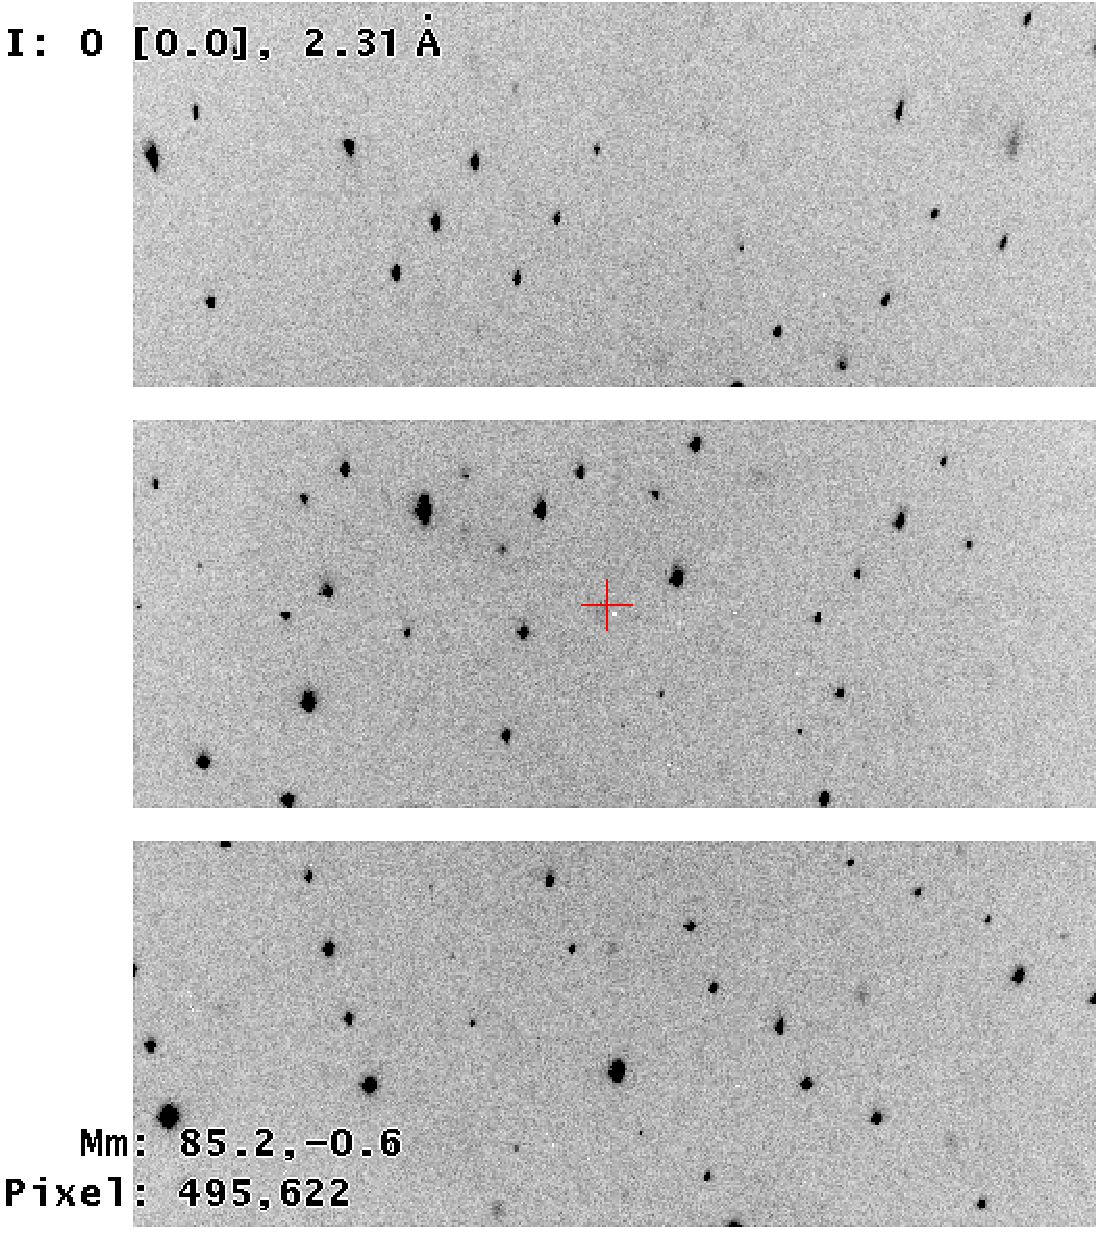
\includegraphics[width=2.5in]{1191_00005}
\caption{\fontsize{15}{21}\selectfont %
Sample Pilatus 300K diffraction image from DLS I19.
Image produced by adxv
}
\label{fig:1191_00005}
\end{center}
\end{wrapfigure}
\\
loop\_\\
{\bf \_diffrn\_detector\_axis.detector\_id}\\
\-\ ~~~{\bf \_diffrn\_detector\_axis.axis\_id}\\
 None DETECTOR\_2THETA\\
 None DETECTOR\_X\\
 None DETECTOR\_Y\\
 None DETECTOR\_Z\\
\\
{\bf \_diffrn\_detector\_element.id} ELEMENT1  
{\bf \_diffrn\_detector\_element.detector\_id}  None \-\\ \\
{\bf \_diffrn\_data\_frame.id}~~FRAME1\\
{\bf \_diffrn\_data\_frame.detector\_element\_id}~~ELEMENT1 \-\\ \\
{\bf \_diffrn\_data\_frame.array\_id}~~ARRAY1~~~~{\bf \_diffrn\_data\_frame.binary\_id} 1\\
{\bf \_diffrn\_scan.id SCAN1  {\bf \_diffrn\_scan.frame\_id\_start} FRAME1\\
{\bf \_diffrn\_scan.frame\_id\_end} FRAME1  {\bf \_diffrn\_scan.frames} 1\\
{\bf \_diffrn\_measurement.diffrn\_id} DLS\_I19  {\bf \_diffrn\_measurement.id} GONIOMETER  \_diffrn\_measurement.number\_of\_axes} 3  {\bf \_diffrn\_measurement.method} rotation\\
{\bf \_diffrn\_measurement.sample\_detector\_distance} 104.00\\
\\
loop\_\\
{\bf \_diffrn\_measurement\_axis.measurement\_id  \_diffrn\_measurement\_axis.axis\_id}\\
 GONIOMETER GONIOMETER\_OMEGA\\
 GONIOMETER GONIOMETER\_KAPPA\\
 GONIOMETER GONIOMETER\_PHI\\
\\
{\bf \_diffrn\_radiation\_wavelength.id} WAVELENGTH1  {\bf \_diffrn\_radiation\_wavelength.wavelength} 0.68890  {\bf \_diffrn\_radiation\_wavelength.wt} 1\\
\\
loop\_\\
{\bf \_diffrn\_scan\_axis.scan\_id}~~{\bf \_diffrn\_scan\_axis.axis\_id}\\
\-\ ~~~{\bf \_diffrn\_scan\_axis.angle\_start}~~{\bf \_diffrn\_scan\_axis.angle\_range}~~{\bf \_diffrn\_scan\_axis.angle\_increment}\\
\-\ ~~~~~~{\bf \_diffrn\_scan\_axis.displacement\_start}  {\bf \_diffrn\_scan\_axis.displacement\_range}\\
\-\ ~~~~~~~~~{\bf \_diffrn\_scan\_axis.displacement\_increment}\\
 SCAN1 GONIOMETER\_OMEGA 23.0000 1.0000 1.0000 0.0 0.0 0.0\\
 SCAN1 GONIOMETER\_KAPPA 70.0000 0.0000 0.0000 0.0 0.0 0.0\\
 SCAN1 GONIOMETER\_PHI -179.0000 0.0000 0.0000 0.0 0.0 0.0\\
 SCAN1 DETECTOR\_2THETA 119.0000 0.0 0.0 0.0 0.0 0.0\\
 SCAN1 DETECTOR\_Z 0.0 0.0 0.0 104.00 0.0 0.0\\
 SCAN1 DETECTOR\_Y 0.0 0.0 0.0 0.0 0.0 0.0\\
 SCAN1 DETECTOR\_X 0.0 0.0 0.0 0.0 0.0 0.0\\
\\
{\bf \_diffrn\_scan\_frame.frame\_id} FRAME1  {\bf \_diffrn\_scan\_frame.frame\_number} 1\\
{\bf \_diffrn\_scan\_frame.integration\_time} 0.997000  {\bf \_diffrn\_scan\_frame.exposure\_time} 1.000000\\
{\bf \_diffrn\_scan\_frame.scan\_id} SCAN1  {\bf \_diffrn\_scan\_frame.date} 2013-08-15T13:21:53.634\\
\\
\vspace{-4mm}%

\begin{minipage}[]{0.525\linewidth}
loop\_\\
{\bf \_diffrn\_scan\_frame\_axis.frame\_id}\\
\-\ ~~{\bf \_diffrn\_scan\_frame\_axis.axis\_id}\\
\-\ ~~~~{\bf \_diffrn\_scan\_frame\_axis.angle}\\
\-\ ~~~~~~{\bf \_diffrn\_scan\_frame\_axis.displacement}\\
FRAME1~GONIOMETER\_OMEGA~23.0~0.0\\
FRAME1~GONIOMETER\_KAPPA~70.0~0.0\\
FRAME1~GONIOMETER\_PHI~-\nobreak{}179.0~0.0\\
FRAME1~DETECTOR\_2THETA~119.0~0.0\\
FRAME1~DETECTOR\_Z~0.0~104.0\\
FRAME1~DETECTOR\_Y~0.0~0.0\\
FRAME1~DETECTOR\_X~0.0~0.0\\
\\
loop\_\\
{\bf \_axis.id~~\_axis.type} \\
\-\ ~~{\bf \_axis.equipment~~\_axis.depends\_on}\\
\-\ ~~~~{\bf \_axis.vector[1]~~\_axis.vector[2]}\\
\-\ ~~~~~~{\bf \_axis.vector[3]}\\
\-\ ~~~~~~~~{\bf \_axis.offset[1]  \_axis.offset[2]}\\
\-\ ~~~~~~~~~~{\bf   \_axis.offset[3]}\\
\end{minipage}\hfill\begin{minipage}[]{0.475\linewidth}
\vspace{-10mm}
\hspace{-40mm}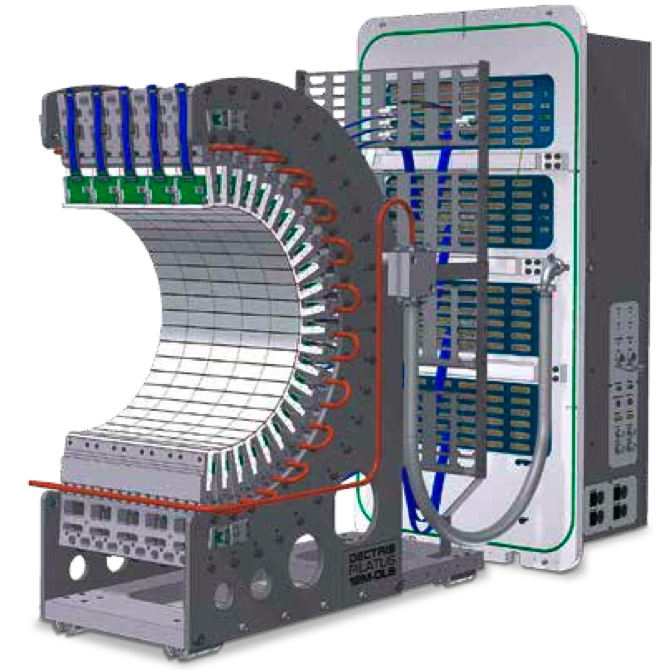
\includegraphics[width=7.5in]{I23}\\
\fontsize{16}{20}\selectfont %
{\bf Figure 3.} Curved DECTRIS detector
for DLS beamline I23, an example of a detector with a complex geometry 
best described using the imgCIF/CBF ontology.  NeXus has now adopted a
similar approach to axis definitions.
\end{minipage}
 GONIOMETER\_OMEGA rotation goniometer . 1 0 0 . . .\\
 GONIOMETER\_KAPPA rotation goniometer \\
 \-\ ~~~~~~~  GONIOMETER\_OMEGA 0.642788 -0.766044 0 . . .\\
 GONIOMETER\_PHI rotation goniometer GONIOMETER\_KAPPA 1 0 0 . . .\\
 SOURCE general source . 0 0 1 . . .\\
 GRAVITY general gravity . 0 -1 0 . . .\\
 DETECTOR\_2THETA rotation detector . 1 0 0 . . .\\
 DETECTOR\_Z translation detector DETECTOR\_2THETA 0 0 -1 0 0 0\\
 DETECTOR\_Y translation detector DETECTOR\_Z 0 -1 0 0 0 0\\
 DETECTOR\_X translation detector DETECTOR\_Y 1 0 0 0 0 0\\
 ELEMENT\_X translation detector DETECTOR\_X 1 0 0 -41.05 52.32 0\\
 ELEMENT\_Y translation detector ELEMENT\_X 0 -1 0 0 0 0\\
\\
loop\_\\
{\bf \_array\_structure\_list.array\_id  \_array\_structure\_list.index}\\
\-\ ~~~{\bf \_array\_structure\_list.dimension  \_array\_structure\_list.precedence}\\
\-\ ~~~~~~~{\bf \_array\_structure\_list.direction  \_array\_structure\_list.axis\_set\_id}\\
 ARRAY1 1 487 1 increasing ELEMENT\_X\\
 ARRAY1 2 619 2 increasing ELEMENT\_Y\\
\\
loop\_\\
{\bf \_array\_structure\_list\_axis.axis\_set\_id  \_array\_structure\_list\_axis.axis\_id}\\
\-\ ~~~{\bf \_array\_structure\_list\_axis.displacement  \_array\_structure\_list\_axis.displacement\_increment}\\
 ELEMENT\_X ELEMENT\_X 0.0 0.1720    ELEMENT\_Y ELEMENT\_Y 0.0 0.1720\\
\\
loop\_\\
{\bf \_array\_element\_size.array\_id  \_array\_element\_size.index  \_array\_element\_size.size}\\
 ARRAY1 1 0.000172   ARRAY1 2 0.000172\\
\\
{\bf \_array\_intensities.array\_id} ARRAY1  {\bf \_array\_intensities.binary\_id} 1\\
{\bf \_array\_intensities.linearity} linear  {\bf \_array\_intensities.gain} 1.0  {\bf \_array\_intensities.gain\_esd} .\\
{\bf \_array\_intensities.overload} 1298839  {\bf \_array\_intensities.undefined\_value} -1\\
\\
{\bf \_array\_structure.id} ARRAY1  {\bf \_array\_structure.encoding\_type} "signed 32-bit integer"\\
{\bf \_array\_structure.compression\_type} none  {\bf \_array\_structure.byte\_order} little\_endian\\

\end{minipage}%
\hspace{10mm}\hfill\begin{minipage}[]{0.29\linewidth}
\section*{Equivalent~HDF5/NeXus~File}

\fontsize{15}{21}\selectfont 
\noindent{}{\bf /:NXroot}\\
\-\ ~~~@creator=``CBFlib''\\
\-\ ~~~@creator\_version=``0.9.5 (r492)  2014-04-27 12:00:40 -0400 (Sun, 27 Apr 2014)''\\
\-\ ~~~{\bf /entry:NXentry}\\
\-\ ~~~~~~{\bf /data:NXdata}\\
\-\ ~~~~~~~~~@axes= [ ``'', ``y'', ``x'' ];~@signal=``data''\\
\-\ ~~~~~~~~~@x\_indices=2; @y\_indices=1\\
\-\ ~~~~~~~~~/data= [11, 11, 13, 13, 11, ...  9, 13, 9, 18\\
\-\ ~~~~~~~~~~~~@signal=1\\
\-\ ~~~~~~~~~/offset =0\\
\-\ ~~~~~~~~~/scaling\_factor=1\\
\-\ ~~~~~~~~~/x= [ 0, 0.172, 0.344, 0.516, ... 83.248, 83.42, 83.592]\\
\-\ ~~~~~~~~~~~~@depends\_on=``/entry/instrument/detector/transformations/DETECTOR\_X''\\
\-\ ~~~~~~~~~~~~@equipment =``detector''; @offset = [41.05, 52.32, 0]; @offset\_units =``mm''\\
\-\ ~~~~~~~~~~~~@transformation\_type =``translation''; @units =``mm''\\
\-\ ~~~~~~~~~~~~@vector= [-1, 0, 0]\\
\-\ ~~~~~~~~~/y= [ 0, 0.172, 0.344, 0.516, ...  105.952, 106.124, 106.296]\\
\-\ ~~~~~~~~~~~~@depends\_on=``/entry/instrument/detector/x\_pixel\_offset''\\
\-\ ~~~~~~~~~~~~@equipment =``detector''; @offset = [0, 0, 0]; @offset\_units =``mm''\\
\-\ ~~~~~~~~~~~~@transformation\_type =``translation''; @units =``mm''\\
\-\ ~~~~~~~~~~~~@vector= [0, -1, 0]\\
\-\ ~~~~~~/definition=``NXmx''\\
\-\ ~~~~~~~~~@version=``1.2''\\
\-\ ~~~~~~{\bf /instrument:NXinstrument}\\
\-\ ~~~~~~~~~/detector:NXdetector\\
\-\ ~~~~~~~~~~~~/count\_time=1;~@units =``s''\\
\-\ ~~~~~~~~~~~~/data~$\rightarrow$~~``/entry/data/data''\\
\-\ ~~~~~~~~~~~~/depends\_on=``/entry/instrument/detector/transformations/DETECTOR\_X''\\
\-\ ~~~~~~~~~~~~/description=``pilatus''\\
\-\ ~~~~~~~~~~~~/distance=104;~@units =``mm''\\
\-\ ~~~~~~~~~~~~/frame\_start\_time=``2013-08-15T13:21:53.634''\\
\-\ ~~~~~~~~~~~~/offset~$\rightarrow$~~``/entry/data/offset''\\
\-\ ~~~~~~~~~~~~/saturation\_value=1298839\\
\-\ ~~~~~~~~~~~~/scaling\_factor $\rightarrow$  ``/entry/data/scaling\_factor''\\
\-\ ~~~~~~~~~~~~{\bf /transformations:NXtransformations}\\
\-\ ~~~~~~~~~~~~~~~/DETECTOR\_2THETA= [119]\\
\-\ ~~~~~~~~~~~~~~~~~~@depends\_on=``.''; @equipment =``detector''; @offset = [0, 0, 0]; @offset\_units =``mm''\\
\-\ ~~~~~~~~~~~~~~~~~~@transformation\_type =``rotation''; @units =``degrees''\\
\-\ ~~~~~~~~~~~~~~~~~~@vector = [-1, 0, 0]\\
\-\ ~~~~~~~~~~~~~~~/DETECTOR\_X = [0]\\
\-\ ~~~~~~~~~~~~~~~~~~@depends\_on=``/entry/instrument/detector/transformations/DETECTOR\_Y''\\
\-\ ~~~~~~~~~~~~~~~~~~@equipment =``detector''; @offset = [0, 0, 0]; @offset\_units =``mm''\\
\-\ ~~~~~~~~~~~~~~~~~~@transformation\_type  = ``translation''; @units = ``mm''\\
\-\ ~~~~~~~~~~~~~~~~~~@vector  = [-1, 0, 0]\\
\-\ ~~~~~~~~~~~~~~~/DETECTOR\_Y = [0]\\
\-\ ~~~~~~~~~~~~~~~~~~@depends\_on=``/entry/instrument/detector/transformations/DETECTOR\_Z''\\
\-\ ~~~~~~~~~~~~~~~~~~@equipment  = ``detector''; @offset  = [0, 0, 0]; @offset\_units  = ``mm''\\
\-\ ~~~~~~~~~~~~~~~~~~@transformation\_type  = ``translation''; @units = ``mm''\\
\-\ ~~~~~~~~~~~~~~~~~~@vector = [0, -1, 0]\\
\-\ ~~~~~~~~~~~~~~~/DETECTOR\_Z = [104]\\
\-\ ~~~~~~~~~~~~~~~~~~@depends\_on=``/entry/instrument/detector/transformations/DETECTOR\_2THETA''\\
\-\ ~~~~~~~~~~~~~~~~~~@equipment =``detector''; @offset = [0, 0, 0]; @offset\_units =``mm''\\
\-\ ~~~~~~~~~~~~~~~~~~@transformation\_type =``translation''; @units =``mm''\\
\-\ ~~~~~~~~~~~~~~~~~~@vector= [0, 0, 1]\\
\-\ ~~~~~~~~~~~~/undefined\_value= [-1]\\
\-\ ~~~~~~~~~~~~/x\_pixel\_offset $\rightarrow$  ``/entry/data/x''\\
\-\ ~~~~~~~~~~~~/x\_pixel\_size=0.172; @units =``mm''\\
\-\ ~~~~~~~~~~~~/y\_pixel\_offset $\rightarrow$  ``/entry/data/y''\\
\-\ ~~~~~~~~~~~~/y\_pixel\_size=0.172; @units =``mm''\\
\-\ ~~~~~~~~~{\bf /monochromator:NXmonochromator}\\
\-\ ~~~~~~~~~~~~/description=``Si 111''\\
\-\ ~~~~~~~~~{\bf /source:NXsource}\\
\-\ ~~~~~~~~~~~~/name=``Diamond Light Source Beamline I19''\\
\-\ ~~~~~~~~~~~~/type =``synchrotron''\\
\-\ ~~~~~~~~~{\bf /transformations:NXtransformations}\\
\-\ ~~~~~~~~~~~~/BEAM = []\\
\-\ ~~~~~~~~~~~~~~~@depends\_on=``.''; @equipment =``general''; @system=``McStas\_absolute''\\
\-\ ~~~~~~~~~~~~~~~@transformation\_type =``general''\\
\-\ ~~~~~~~~~~~~~~~@vector= [0, 0, 1]\\
\-\ ~~~~~~~~~~~~/GRAVITY= []\\
\-\ ~~~~~~~~~~~~~~~@depends\_on=``.''; @equipment =``general''; @system=``McStas\_absolute''\\
\-\ ~~~~~~~~~~~~~~~@transformation\_type =``general''\\
\-\ ~~~~~~~~~~~~~~~@vector= [0, -1, 0]\\
\-\ ~~~~~~~~~~~~/SOURCE= []\\
\-\ ~~~~~~~~~~~~~~~@depends\_on=``.''; @equipment =``general''; @system=``McStas\_absolute''\\
\-\ ~~~~~~~~~~~~~~~@transformation\_type =``general''\\
\-\ ~~~~~~~~~~~~~~~@vector= [0, 0, -1]\\
\-\ ~~~~~~~~~~~~/UP= []\\
\-\ ~~~~~~~~~~~~~~~@depends\_on=``.''; @equipment =``general''; @system=``McStas\_absolute''\\
\-\ ~~~~~~~~~~~~~~~@transformation\_type =``general''\\
\-\ ~~~~~~~~~~~~~~~@vector= [0, 1, 0]\\
\-\ ~~~~~~/method=``rotation''\\
\-\ ~~~~~~{\bf /sample:NXsample}\\
\-\ ~~~~~~~~~{\bf /beam:NXbeam}\\
\-\ ~~~~~~~~~~~~/incident\_divergence\_x= [0.08]; @units =``degrees''\\
\-\ ~~~~~~~~~~~~/incident\_divergence\_xy= [0]; @units =``degrees\^2''\\
\-\ ~~~~~~~~~~~~/incident\_divergence\_y= [0.01]; @units =``degrees''\\
\-\ ~~~~~~~~~~~~/incident\_polarisation\_stokes= [1, 0.8, 0, 0]\\
\-\ ~~~~~~~~~~~~/incident\_wavelength=0.6889; @units =``angstroms''\\
\-\ ~~~~~~~~~~~~/weight=1\\
\-\ ~~~~~~~~~/depends\_on=``/entry/sample/transformations/GONIOMETER\_PHI''\\
\-\ ~~~~~~~~~{\bf /transformations:NXtransformations}\\
\-\ ~~~~~~~~~~~~/GONIOMETER\_KAPPA= [70]\\
\-\ ~~~~~~~~~~~~~~~@depends\_on=``/entry/sample/transformations/GONIOMETER\_OMEGA''\\
\-\ ~~~~~~~~~~~~~~~@equipment =``goniometer''; @offset = [0, 0, 0]; @offset\_units =``mm''\\
\-\ ~~~~~~~~~~~~~~~@transformation\_type =``rotation''; @units =``degrees''\\
\-\ ~~~~~~~~~~~~~~~@vector= [-0.642788, -0.766044, 0]\\
\-\ ~~~~~~~~~~~~/GONIOMETER\_OMEGA= [23]\\
\-\ ~~~~~~~~~~~~~~~@depends\_on=``.''; @equipment =``goniometer''; @offset = [0, 0, 0]; @offset\_units =``mm''\\
\-\ ~~~~~~~~~~~~~~~@transformation\_type =``rotation''; @units =``degrees''\\
\-\ ~~~~~~~~~~~~~~~@vector= [-1, 0, 0]\\
\-\ ~~~~~~~~~~~~/GONIOMETER\_PHI= [-179]\\
\-\ ~~~~~~~~~~~~~~~@depends\_on=``/entry/sample/transformations/GONIOMETER\_KAPPA''\\
\-\ ~~~~~~~~~~~~~~~@equipment =``goniometer''; @offset = [0, 0, 0]; @offset\_units =``mm''\\
\-\ ~~~~~~~~~~~~~~~@transformation\_type =``rotation''; @units =``degrees''\\
\-\ ~~~~~~~~~~~~~~~@vector= [-1, 0, 0]\\
\vspace{-9mm}
\begin{itemize}

\item{{\bf The minimum required NeXus application definition for single crystal 
monochromatic macromolecular crystallography is given in the NXmx application
definition}:

{\fontsize{18}{22}\selectfont \url{http://download.nexusformat.org/sphinx/classes/contributed_definitions/NXmx.html}}
}
\end{itemize}


 
\vspace{-12mm}
%\bibliographystyle{plain}
%\bibliographystyle{wmaainf}
\bibliographystyle{phcpc}
\bibliography{Integration_Poster}

\vspace{-12mm}
\section*{Acknowledgements}

Our  thanks  to  James  Hester,  Chair  of  COMCIFS and  
Mark   Koennecke,   Chair   of   NIAC,   for   supporting  
and  encouraging  this  effort  and  to  all  participants  
in   COMCIFS   and  NIAC  for  helpful  comments.  Our thanks 
to   Nick   Sauter   and   Aaron Brewster  for  extending  
this  work  to  CSPAD.  Our  thanks  for  years  of  supporting  
efforts  at  the  BNL  PXRR  Group:  Robert  M.  Sweet,  Dieter  Schneider,  
Howard   Robinson,   John   Skinner,   Matt   Cowan,  
Leonid  Flaks,  Richard  Buono;  at DLS:  Alun  Ashton,  
Bill  Pulford;  and  at  the  Dowling  College  ARCiB  Lab  
Group: Mojgan   Asadi,   Kostandina   Bardhi, Keti Bardhi  
Limone  Rosa, Our   thanks   to  DECTRIS,   BIOIHDF and   the HDF  
Group.  Our  thanks  to  Frances  C.  Bernstein.
This   work  was  funded   in   part   by   NIGMS,   DOE,  
NSF,   PaNdata   ODI   (EU   7th   Framework  
Programme).
\end{minipage}\hfill

\vfill
\end{document}  
